\documentclass[../main.tex]{subfiles}

\begin{document}

\section{Results}

	\subsection{Structural Models}
	\begin{table}[t]
		\centering
		\caption{Model Fit Indices}
		\begin{tabular*}{1\textwidth}{@{\extracolsep{\fill}} l c c c c c @{}}
			Model   & $\chi^{2}$  & \textit{df} & CFI & TLI & RMSEA \\ \hline
			CFA     & 33.92*** & 9  & .96 & .93 & .07   \\
			MIMIC 1 & 68.72*** & 29 & .94 & .91 & .05   \\
			MIMIC 2 & 68.00*** & 29 & .94 & .91 & .05   \\ \hline
			***$p<.001$.
		\end{tabular*}
		\label{tab:fit}
	\end{table}

	Our first model, the CFA on the shortened AEQ, resulted in a validation of the shortened questionnaire. The model fit can be seen in Table~\ref{tab:fit} under CFA. All fit indices, apart from the conservative $\chi^{2}$, were in the acceptable range (i.e., $>.90$ for CFI and TLI, and $<.08$ for RMSEA). All standardized factor loadings from the latent variable on the measured indices were significant ($p<.001$) and strong enough to justify interpretation (>.80). We interpret these results as evidence for our shortened version of the AEQ being adequate for measuring an individual's aesthetic experience.
	
	For our first MIMIC model, we also obtained good fit measures, as seen in Table~\ref{tab:fit} under MIMIC 1. This model included an effect of sex, age, and nationality on aesthetic experience, and an effect of sex, age, and nationality on the proportion of agreement with the GAN. While the measurement part of the model remained largely unchanged, the new structural part of the model only showed a significant effect of nationality on aesthetic experience ($\beta = 0.01, p<.05$). This finding may have consequences for the AEQ itself, as \textcite{wanzerExperiencingFlowViewing2020} had mentioned that their own sample only included US participants. On the other hand, we did not find an effect of age and sex on aesthetic experience, unlike \textcite{wanzerExperiencingFlowViewing2020}. The most important finding here is that there was no effect of the latent aesthetic experience on the behavioral outcome variable of aesthetic judgement, which has important implications for the rest of our study.
	
	For our second MIMIC model, illustrated in Figure~\ref{fig:finalmodel}, we made changes on theoretical bases. The fit indices were equally good, as seen in Table~\ref{tab:fit} under MIMIC 2, but we believe this second model makes more sense from a theoretical point of view. The standardized factor loadings were again very similar. Again, the effects of age and sex on aesthetic experience and aesthetic judgement were not significant. Nationality still has a significant effect on aesthetic experience here, but not on the cultural indicator. There was also no significant effect of aesthetic experience on aesthetic judgement here.

	\begin{figure}[t]
		\caption{Final MIMIC Model}
		\label{fig:finalmodel}
		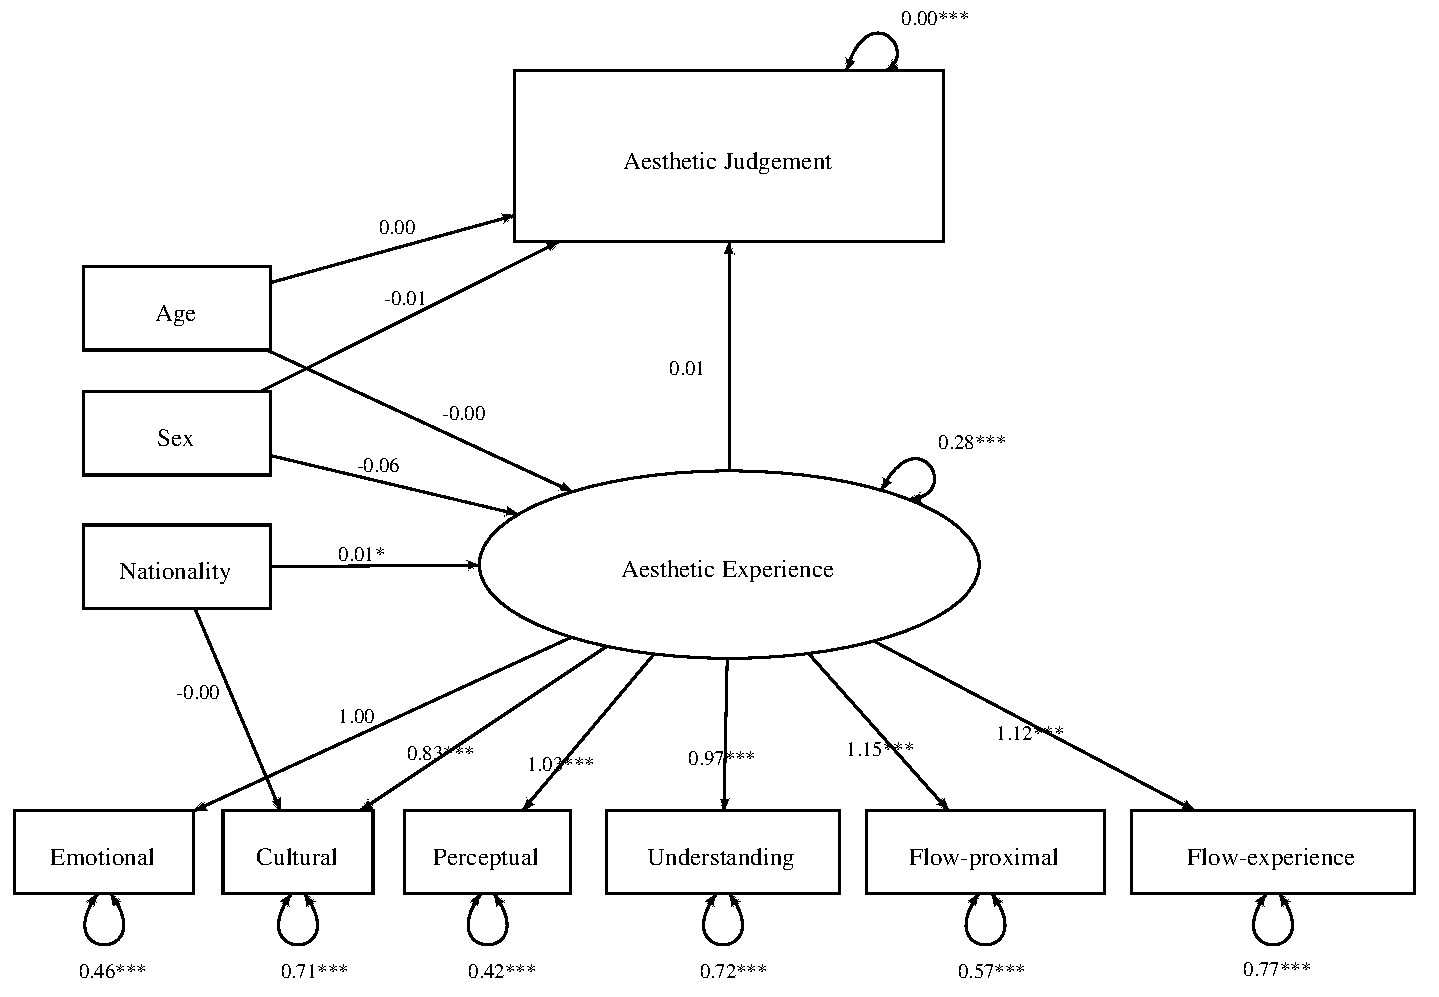
\includegraphics[width=1\linewidth]{images/model3.pdf}
	\end{figure}

	We can interpret these results as there being no effect of a person's demographic characteristics and their aesthetic experience on the outcome of the behavioral image rating task. This implies that the simple image comparison we used in our experiment is not influenced by seemingly relevant factors, pointing to a potential universal nature of aesthetic appreciation of the images we provided in the task. Furthermore, this will make our interpretations of the factors determining the aesthetic value of an image through GANalyze more generalizable.
	


	\subsection{Behavioral Task}
	Figure~\ref{fig:psychometric_curves} shows the proportion of responses in correspondence with GANalyze's generated images for all participants.

	\begin{figure}[ht]
		\caption{Psychometric Function for Image Discrimination}
		\label{fig:psychometric_curves}
		\centering
		\begin{subfigure}{0.45\textwidth}
			\centering
			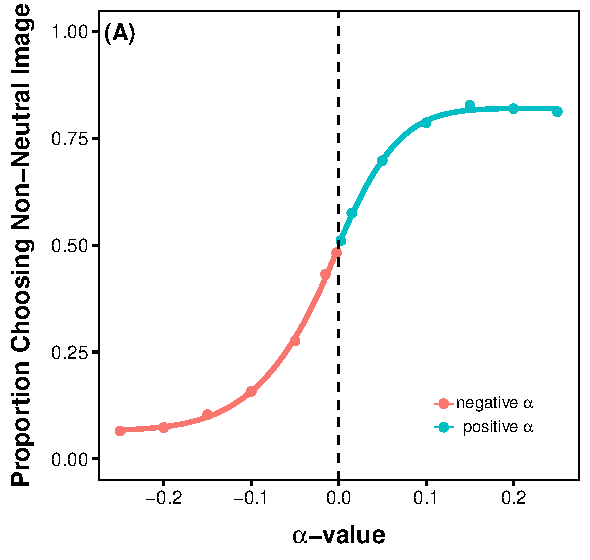
\includegraphics[width=1\linewidth]{results/cont_asym.pdf}
			\caption{\centering One big caption somehow}
		\end{subfigure} \hfill
		\begin{subfigure}{0.45\textwidth}
			\centering
			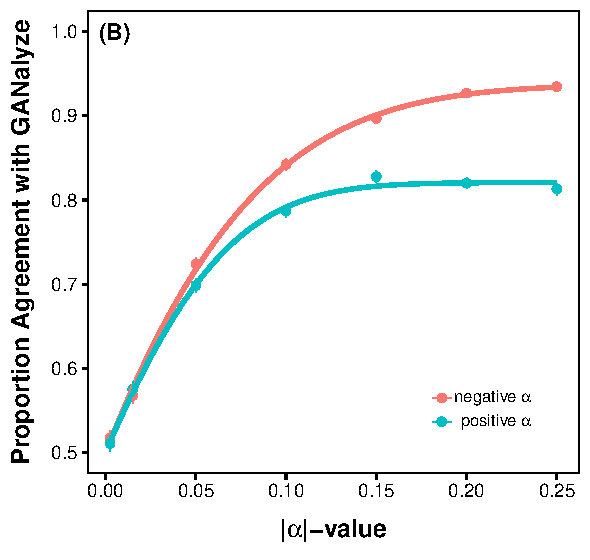
\includegraphics[width=1\linewidth]{results/alpha_correct.pdf}
			\caption{\centering a}
		\end{subfigure} \hfill
	\end{figure}


\end{document}